\chapter{A Gaussian mixture model}\label{ch:gmm}
In \Cref{ch:linear_theory}, we described and justified a framework for computing approximations to the solutions of non-linear SDEs via linearisations about solutions to the corresponding deterministic system.
A key advantage of this approximation is efficiency of computation; rather than having to generate a large number of realisations of the SDE solution to understand, either qualitatively or for the purposes of inference and estimation, the probability distribution of the solution, we can solve a smaller system of differential equations to obtain the first two moments.
When the initial condition is fixed or Gaussian, the resulting linearisation solution is a Gaussian process, providing an approximation characterised \emph{entirely} by these two moments.
A Gaussian approximation has further advantages, leading to its use across many different applications \citep{KaszasHaller_2020_UniversalUpperEstimate,ArchambeauEtAl_2007_GaussianProcessApproximations,Jazwinski_2014_StochasticProcessesFiltering,SarkkaSolin_2019_AppliedStochasticDifferential,Sanz-AlonsoStuart_2017_GaussianApproximationsSmall}.
For example, even in inference requiring Monte-Carlo simulations, a Gaussian distribution with a specified mean and covariance is faster to sample from than generating numerical solutions of the nonlinear SDE.

Recall that we are interested in approximating the solution at a time \(t\) to the nonlinear stochastic differential equation
\begin{equation}
	\dif y_t = u\!\left(y_t, t\right)\dif t + \epsilon\sigma\!\left(y_t, t\right)\dif W_t,
	\label{eqn:sde_y_gmm}
\end{equation}
subject to some random initial condition \(y_s = x\), by using solutions of the corresponding deterministic system
\begin{equation}
	\dod{F_s^t\!\left(x_0\right)}{t} = u\!\left(F_s^t\!\left(x\right), t\right), \quad F_s^s\!\left(x\right) = x.
	\label{eqn:det_ode_gmm}
\end{equation}
The behaviour of the solution \cref{eqn:sde_y_gmm} over the time interval \((s,t)\) for small \(\epsilon\) can be approximated by the linearised SDE
\begin{equation}
	\dif l_t = \left(u\!\left(F_s^t\!\left(x\right), t\right) + \nabla u\!\left(F_s^t\!\left(x\right), t\right)\left[l_t - F_s^t\!\left(x\right)\right]\right)\dif t + \epsilon\sigma\!\left(F_s^t\!\left(x\right), t\right)\dif W_t,
	\label{eqn:sde_linear_gmm}
\end{equation}
subject to the initial condition \(l_s = x\).
The theory in \Cref{ch:linear_theory} considered the evolution of \cref{eqn:sde_y_gmm} over a time interval \((0,t)\) and subject to some initial condition at time \(0\).
However, by using a simple time shift our theory can be applied to any finite time interval \((s,t)\), where the solution is specified at time \(s\) instead of \(0\), without loss of generality.
Note that we have now also dropped the dependence of \(\epsilon\) in the notation \(y_t\) and \(l_t\), as \(\epsilon\) is now treated as a fixed value specified as part of the model.
Suppose that the initial condition \(x\) follows a Gaussian distribution with mean \(x_0\) and a specified covariance matrix \(\Sigma_s\).
If the initial condition is fixed as \(x_s\), then we set \(\Sigma_s = O\), the \(n \times n\) zero matrix, so that the initial distribution is a Dirac delta.
We will focus our attention on this case for the remainder of this thesis, having already provided a general framework in \Cref{ch:linear_theory} for other initial conditions.
By taking the mean \(x_s\) as the initial condition to \cref{eqn:det_ode_gmm}, we ensure that the initial uncertainty (measured by the \(L_r\)-norm as in \Cref{ch:linear_theory}) scales with the trace of \(\Sigma_s\).
The solution to \cref{eqn:sde_linear_gmm} is then a Gaussian process characterised by the mean \(F_s^t\!\left(x_0\right)\) and covariance matrix \(\var{l_t}\), for which explicit expressions for are given in \Cref{cor:limit_moments}.
For notational brevity, set \(w_t \equiv F_s^t\!\left(x_s\right)\) and \(\Pi_t \equiv \var{l_t}\).
When the Jacobian \(\nabla u\) of the vector field \(u\) is available, or can approximated appropriately, the moments of the Gaussian solution can be obtained by the system of ordinary differential equations
\begin{subequations}\label{eqn:gauss_de}
	\begin{align}
		\dod{w_t}{t}   & = u\!\left(w_t, t\right), \quad w_s = x_0 \label{eqn:gauss_mean_de}                                                                                                           \\
		\dod{\Pi_t}{t} & = \begin{multlined}[t]
			                   \nabla u\!\left(w_t, t\right) \Pi_t + \Pi_t\left[\nabla u\left(w_t, t\right)\right]^{\T} + \sigma\left(w_t, t \right)\sigma\left(w_t, t\right)^{\T}, \quad \Pi_s = \Sigma_s.
		                   \end{multlined}
		\label{eqn:gauss_cov_de}
	\end{align}
\end{subequations}
In practice, \cref{eqn:gauss_de} must be solved numerically, but can be more computationally efficient than the alternative of generating many realisations of \cref{eqn:sde_y_gmm}.
Thus, we can efficiently compute a Gaussian approximation \(\Gauss{w_t, \Sigma_t}\) to the solution to the nonlinear SDE \cref{eqn:sde_y_gmm} at time \(t\) by solving \cref{eqn:gauss_de} only.
The \citet{Mazzoni_2008_ComputationalAspectsContinuous} method, outlined in \Cref{sec:mazzoni}, provides a computationally efficient algorithm for solving \Cref{eqn:gauss_de} jointly.

Although computationally appealing, this Gaussian approximation is only `reasonable' in the limit of small initial and ongoing uncertainty, which we quantified exactly with the bound in \Cref{thm:main}, and demonstrated heuristically with examples in \Cref{fig:sine_hists,fig:1d_mult_hists,fig:y_hists}.
In practice, the scale of the noise is an inherent part of a model and there is no guarantee that it is sufficiently small for Gaussian approximations to be reasonable.
When the noise scale is larger, we see non-Gaussianity emerge---the numerical solutions in \Cref{fig:sine_hists,fig:1d_mult_hists,fig:y_hists} exhibit skewness, bi-modality, and other departures from Gaussianity.
Non-Gaussianity is also often observed in statistical measurements in practice, such as in atmospheric regimes \citep{SuraEtAl_2005_MultiplicativeNoiseNonGaussianity}, experimental fluid flows \citep{del-Castillo-Negrete_1998_AsymmetricTransportNonGaussian}, and oceanic flows \citep{BraccoEtAl_2000_VelocityProbabilityDensity}.
Although the Gaussian approximation can still provide qualitative insight into the behaviour of these solutions (see stochastic sensitivity, for instance), to produce a reasonable approximation we need a method that can capture these departures from Gaussianity.

% \section{An example: Ben\^e's SDE}
\begin{figure}
	\centering
	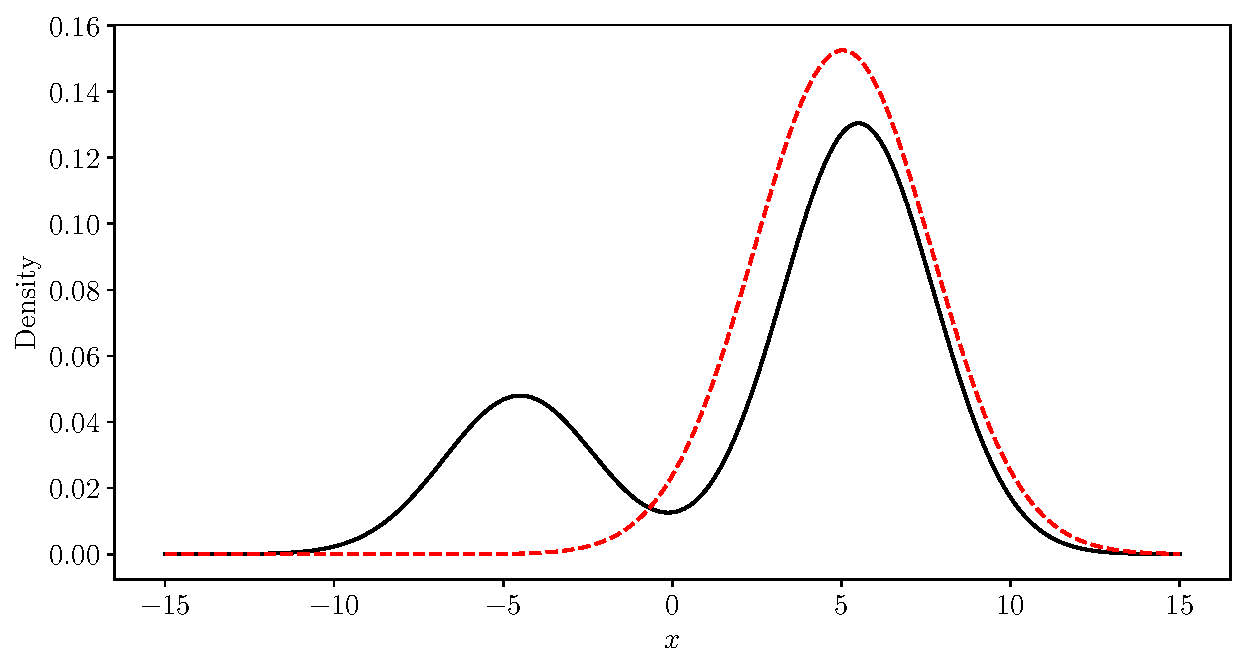
\includegraphics[width=0.9\textwidth]{chp05_gmm/figures/bene_final_gauss_5.0.pdf}
	\caption{The probability density function \cref{eqn:bene_sde_pdf} of the solution \(x_5\) (in black) to Ben\^e's SDE \cref{eqn:bene_sde}, with fixed initial condition \(x_0 = 1/2\).
		The density function of the Gaussian solution to the corresponding linearisation is overlaid in dashed red.}
	\label{fig:bene_gauss}
\end{figure}

To further illustrate this point, we consider another example of a 1-dimensional stochastic differential equation.
Ben\^e's SDE \citep{SarkkaSolin_2019_AppliedStochasticDifferential} is
\begin{equation}
	\dif x_t = \tanh\!\left(x_t\right)\dif t + \dif W_t.
	\label{eqn:bene_sde}
\end{equation}
In this example we are implicitly taking \(\epsilon = 1\), which is a larger noise scale than we typically expect to apply our results to.
However, this example is purely demonstrative to highlight a limitation of Gaussian approximations and show the potential of the algorithm we are about to propose; later examples will involve a smaller noise scale.
The deterministic system corresponding to \cref{eqn:bene_sde} is
\begin{equation}
	\dod{F_s^t\!\left(x\right)}{t} = \tanh\!\left(F_s^t\!\left(x\right)\right), \quad F_s^s\!\left(x\right) = x,
	\label{eqn:bene_ode}
\end{equation}
which includes an unstable fixed point at \(0\).
The solution to \cref{eqn:bene_ode} over the time interval \((s,t)\) is
\begin{equation}
	F_s^t\!\left(x\right) = \arcsinh\!\left(e^{t-s}\sinh\!\left(x\right)\right).
	\label{eqn:bene_ode_sol}
\end{equation}
We consider the solution to \cref{eqn:bene_sde} subject to the fixed initial condition \(x_0 = 1/2\) and at time \(t = 5\).
The probability density function of the weak solution to \cref{eqn:bene_sde} can be derived using an appropriate change of measure with Girsanov's theorem (see Section 7.3 of \citet{SarkkaSolin_2019_AppliedStochasticDifferential}.
The probability density function for the solution \(x_t\) at time \(t = 5\) is given by
\begin{equation}\label{eqn:bene_sde_pdf}
	p(x) = \frac{1}{\sqrt{10\pi}}\frac{\cosh\left(x\right)}{\cosh\!\left(\frac12\right)}\exp\left[-\frac{5}{2} - \frac{1}{10}\left(x - \frac12\right)^2\right],
\end{equation}
and is plotted in black in \Cref{fig:bene_gauss}.
The density is not symmetric with two distinct modes that result from the unstable fixed point of \cref{eqn:bene_ode} at \(x = 0\).
Many stochastic trajectories are driven away from zero, resulting in the predominant mode centred at \(x = 5.5\).
However, when the stochastic perturbations force a trajectory through the fixed point and into negative values, they are pushed further in the negative direction, leading to the second mode at \(x = -4.5\).
Nonetheless, we can linearise \cref{eqn:bene_sde} about the deterministic trajectory \(F_0^t\!\left(1/2\right)\) solving \cref{eqn:bene_ode} to obtain a Gaussian approximation.
In general, ...
\[
	\dif l_t = \left(\tanh\!\left(F_s^t\!\left(x_0\right)\right) + \arcsech\!\left(F_0^t\!\left(x_0\right)\right)\left[l_t - F_s^t\!\left(x_0\right)\right]\right)\dif t + \dif W_t
\]
with the deterministic flow map \(F_s^t\) given by \cref{eqn:bene_ode_sol}.

Since the deterministic flow map is available analytically in \cref{eqn:bene_ode_sol}, we can determine the variance \(\var{l_t}\) of the solution to the linearised SDE exactly by evaluating \cref{eqn:pi_expl_eqn}.
More generally, when the SDE is linearised over the time interval \([s,t]\) about the trajectory \(F_s^t\!\left(x_s\right)\), the variance is
\[
	\var{l_t} = \frac{2\sinh^2\!\left(x_0\right)\left(t - s\right) + e^{2t - 2s} - 1}{2\sinh^2\!\left(x_0\right) + 2e^{2s - 2t}}
\]
The details of this computation are provided in \Cref{app:bene_calculations}.
\td{A sentence explaining the approximation to this specific initial condition}
The solution to \cref{eqn:bene_sde} at time \(t\) is then approximated by the Gaussian distribution
\[
	\mathcal{N}\!\left(\arcsinh\!\left(e^t \sinh\!\left(1/2\right)\right),\, \frac{2\sinh^2\!\left(1/2\right)t + e^{2t} - 1}{2\sinh^2\!\left(1/2\right) + 2e^{-2t}}\right)
\]
We plot the density of this Gaussian approximation in dashed red in \Cref{fig:bene_gauss}.
The Gaussian approximation cannot capture the bimodality of the true solution, and so only a single mode is captured.
This is a significant limitation of using a single linearisation approximation, which cannot possibly capture any multimodality.
% However, to compensate for the additional negative mode, the mean of the Gaussian approximation is less than that of the positive mode, and the variance is larger.\lb{Again, need to be more precise here. Have a look at the conditional probabilities and compare - the deterministic trajectory would have no idea about the fixed point. Otherwise could omit this sentence - keep it simple, the main point is the bimodality}


% \newcommand{\plotbenepdf}[2]{
% 	\begin{tikzpicture}\begin{axis}[
% 				ymin=0.0,
% 				xmin=-10.0,
% 				xmax=10.0,
% 				axis lines=center,
% 				axis on top=true,
% 				domain=-10:10,
% 				ylabel=$p$,
% 				xlabel=$x$,
% 				ytick=\empty,
% 				yticklabels={},
% 			]
% 			\addplot [mark=none,draw=black,thick,samples=500] {cosh(\x)*exp(-#2/2-1/(2 * #2)*(\x-#1)^2)/((2 * pi * #2)^(1/2) * cosh(#1))};
% 		\end{axis}
% 	\end{tikzpicture}
% }

% \begin{figure}
% 	\begin{center}
% 		\begin{subfigure}{0.49\textwidth}
% 			\plotbenepdf{1/2}{1}
% 			\caption{\(t = 1\)}
% 			\label{fig:bene_1}
% 		\end{subfigure}
% 		\begin{subfigure}{0.49\textwidth}
% 			\plotbenepdf{1/2}{2.5}
% 			\caption{\(t = 2.5\)}
% 			\label{fig:bene_2.5}
% 		\end{subfigure}
% 		\begin{subfigure}{0.49\textwidth}
% 			\plotbenepdf{1/2}{5}
% 			\caption{\(t = 5\)}
% 			\label{fig:bene_5}
% 		\end{subfigure}
% 		\begin{subfigure}{0.49\textwidth}
% 			\plotbenepdf{1/2}{7.5}
% 			\caption{\(t = 7.5\)}
% 			\label{fig:bene_7.5}
% 		\end{subfigure}
% 	\end{center}
% 	\caption{The probability density function \cref{eqn:bene_sde_pdf} for the time-marginal solution of Ben\^e's SDE \cref{eqn:bene_sde}, for the initial condition \(x_0 = 1/2\) at various times.
% 		The density function consists of two distinct modes that move further apart as \(t\) increases.}
% 	\label{fig:bene_pdf}
% \end{figure}



We seek a scheme that can capture departures from Gaussianity in the SDE solution, while still taking advantage of the efficient computation of the corresponding deterministic system and the linearisation approximation.
An alternative perspective of the linearisation solution is that it captures the behaviour of stochastic fluctuations close to a deterministic trajectory, in a similar sense to how a Taylor polynomial captures local behaviour of a nonlinear function.
By `piecing' together several of these approximations together we can capture the stochastic behaviour in different regions of the state space.
A Gaussian mixture model (GMM) provides a framework for combining multiple Gaussian densities into a single distribution, and is therefore the obvious choice for constructing non-Gaussian densities out of our Gaussian approximations.
In this chapter, we outline an algorithm that uses \emph{multiple} Gaussian approximations resulting from the linearised SDE in a mixture model to provide a non-Gaussian approximation to the nonlinear SDE solution.
The algorithm itself is provided in \Cref{sec:gmm_alg}.

% Helper functions for TikZ pic
\newcommand{\TikZGauss}[3]{1 / sqrt(2 * pi * #3) * exp(-(#1 - #2) * (#1 - #2) / #3)} % Args: variable, mean, variance
\newcommand{\TikZMixtureTwo}[8]{% Args: width, comp1_mean, comp1_var, comp2_mean, comp2_var, comp1_weight, comp2_weight, vertical scaling
	\begin{tikzpicture}
		% Two components
		\draw[domain=0:#1, smooth, variable=\x, dashed] plot ({\x}, {#8 * \TikZGauss{\x}{#2}{#3}});
		\draw[domain=0:#1, smooth, variable=\x, dashed] plot ({\x}, {#8 * \TikZGauss{\x}{#4}{#5}});
		% Mixture model
		\draw[domain=0:#1, smooth, variable=\x, very thick] plot ({\x}, {#8 * #6 * \TikZGauss{\x}{#2}{#3} + #8 * #7 * \TikZGauss{\x}{#4}{#5}});
		\draw[thick] (0,0)--(#1,0);
	\end{tikzpicture}
}

\begin{figure}
	\centering
	\begin{subfigure}{0.49\textwidth}
		\TikZMixtureTwo{7}{2}{1}{3}{2}{0.5}{0.5}{3}
		\caption{Skewness}
	\end{subfigure}
	\begin{subfigure}{0.49\textwidth}
		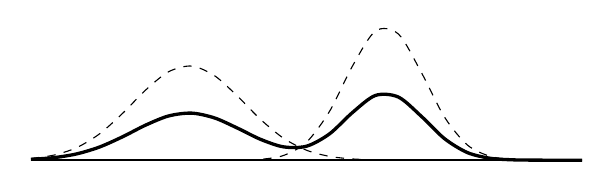
\begin{tikzpicture}
			\TikZMixtureTwo{7}{2}{1}{4.5}{0.5}{0.5}{0.5}{3}
		\end{tikzpicture}
		\caption{Bimodality}
	\end{subfigure}
	\caption{The probability density functions of two Gaussian mixture models in 1-dimension both using two equally weighted components.
		When individual components (dashed) are combined to produce non-Gaussian mixture densities (solid), they can exhibit both (a) skewness and (b) bimodality.}
	\label{fig:mixture_model}
\end{figure}

In general, a Gaussian mixture model with \(K\) components is a probability density function of the form
\[
	p(z) = \sum_{k=1}^{K}{\omega_k \Gauss{z;\, \mu^{(k)}, \Sigma^{(k)}}},
\]
which consists of \(K\) Gaussian components \(\Gauss{\mu^{(k)}, \Sigma^{(k)}}\) with respective weights \(\omega_1, \dotsc, \omega_K \geq 0\) satisfying \(\sum_{k=1}^{K}\omega_k = 1\).
With sufficient components, a Gaussian mixture model can recreate any probability distribution in \(\R^n\) while having many of the properties that make Gaussian distributions appealing in practice \citep{McLachlanEtAl_2019_FiniteMixtureModels}.
\Cref{fig:mixture_model} shows two examples of Gaussian mixture models in 1-dimension, where departures from Gaussianity such as multimodality and skewness can be captured with an appropriate combination of components.


\td{Show more of the computations}
% \begin{figure}
% 	\begin{center}
% 		\begin{tikzpicture}
% 			\draw[scale=2, domain=-3:4, smooth, variable=\x, dashed] plot ({\x}, {exp(-(\x + 0.5) * (\x + 0.5))});
% 			\draw[scale=2, domain=-3:4, smooth, variable=\x, dashed] plot ({\x}, {1 / (sqrt(2 * pi * 0.8))*exp(-(\x - 1.5) * (\x - 1.5) / 0.8)});
% 			\draw[scale=2, domain=-3:4, smooth, variable=\x, thick] plot ({\x}, {0.5 * exp(-(\x + 0.5) * (\x + 0.5)) + 0.5 * 1 / (sqrt(2 * pi * 0.8))*exp(-(\x - 1.5) * (\x - 1.5) / 0.8)});
% 			\draw[->,thick] (-6,0)--(8,0) node[right]{\(x\)};
% 		\end{tikzpicture}
% 		\caption{An example of the probability density function of a Gaussian mixture model with two weighted components.
% 		The two individual components (dashed) are combined to produce the non-Gaussian mixture density (solid).}
% 		\label{fig:mixture_model}
% 	\end{center}
% \end{figure}


% We have a ``local'' approximation for the SDE \cref{eqn:sde_no_eps}, in that solutions to the linearised equation capture the solution behaviour nearby a given deterministic trajectory.
% In practice, the solution to stochastic differential equations are non-Gaussian.
% A key observation of \Cref{sec:theory_gauss} is that the solution to the linearised SDE is Gaussian when the initial condition is Gaussian.
% Through a mixture model, we can capture this non-Gaussianity (leading to a better approximation) while still taking advantage of the computationally efficiency of the Gaussian approximation.




\section{The GMM algorithm}\label{sec:gmm_alg}
Let us now return to the original aim of this chapter: to approximate the SDE solution with a Gaussian mixture model while taking advantage of the computationally efficiency of the Gaussian linearisation approximation.
Given a Gaussian component at a time \(s\), we can `propagate' the component forward to a later time \(t\) by solving \Cref{eqn:gauss_de} initialised with the component mean and covariance matrix.
That is, we are updating the mean and covariance of the Gaussian component by approximating the solution to the original SDE \cref{eqn:sde_y_gmm} over \((s,t)\) with a linearisation about the deterministic trajectory initialised from the component mean.
Given a mixture model with multiple Gaussian components, we can propagate each component separately to update the full model through time in a computationally efficient manner.

\begin{figure}
	\centering
	\begin{tikzpicture}

	\end{tikzpicture}
	\caption{The splitting of a mean \(x\) and covariance matrix \(\Sigma\) into sigma points.}
	\label{fig:sigma_points_ex}
\end{figure}

Our proposed method is ad-hoc and based on a simple intuition: the Gaussian solution provides a reasonable approximation for the local behaviour of the true SDE solution over a short timeframe, but once this is no longer the case, we can capture departures from Gaussianity by introducing more components into the mixture model.
We expect heuristically that as the number of components increase, the full mixture model should provide a closer approximation of the SDE solution density, provided that the components are appropriately placed.
However, our goal is to provide a numerically efficient algorithm, so we wish to minimise the number of components and use the Gaussian approximation whereever possible.
We therefore propose propagating Gaussian components forward through the linearisation model until are no longer reasonable approximations of the local solution behaviour.
Then, we replace violating component with several smaller judiciously chosen components and propagate each new component individually.
We term this the \emph{splitting} step, where a Gaussian component is split into several smaller ones.
The new components should be chosen in such a way as to preserve the original component, which can be achieved as follows.
Let \(\Xi\) follow a Gaussian mixture density with \(N\) components, with respective weights \(w^{(1)}, \dotsc, w^{(N)}\), means \(\mu^{(1)},\dotsc,\mu^{(N)}\), and covariance matrices \(\Sigma^{(1)},\dotsc,\Sigma^{(N)}\).
The variance of the mixture model is then
\begin{align*}
	\var{\Xi} & = \sum_{i=1}^{N}{w^{(i)}\Sigma^{(i)}} + \sum_{i=1}^{N}{w^{(i)}\left(\mu^{(i)} - \bar{\mu}\right)\left(\mu^{(i)} - \bar{\mu}\right)^{\T}} \\
	          & = \text{Mean of covariances} + \text{Covariance of means},
\end{align*}
where \(\bar{\mu} = \sum_{i=1}^{N}{w^{(i)}\mu^{(i)}}\).
This decomposition suggests, at least heuristically, that we can include additional uncertainty (in the form of contributions to the overall variance) within the component means themselves.
By replacing a single component with points, we can ``preserve'' the mean and covariance of the component while introducing additional components that can closer match the non-Gaussian distribution we are seeking to approximate.
This leads to the following condition on how a component is split: the splitting points should be chosen so that
\begin{equation}
	\sum_{i=1}^K{\hat{w}_k x^{(k)}} = x, \quad \sum_{i=1}^{K}{\hat{w}_k\left(x^{(k)} - x\right)\!\left(x^{(k)} - x\right)^{\T}} = \Sigma_0.
	\label{eqn:cov_split_points}
\end{equation}
with weights \(\hat{w}_1,\dotsc,\hat{w}_K > 0\) satisfying \(\sum_{k=1}^{K}{\hat{w}_k} = 1\).
This ensures that the mean and covariance of the original Gaussian is preserved within the (sample) mean and covariance of the new points themselves.
Note that at least \(K = n + 1\) points are necessary for \cref{eqn:cov_split_points} to be satisfied.
The selection of splitting points are similar to the notion of `sigma points', employed in the unscented transform to encode an initial mean and covariance \citep{Uhlmann_1995_DynamicMapBuilding,JulierEtAl_2000_NewMethodNonlinear}.
Any such sigma points satisfy \cref{eqn:cov_split_points}---Table I in \citet{MenegazEtAl_2015_SystematizationUnscentedKalman} provides a list of sigma points and their weightings used across other literature (and reviewed in the context of Kalman filtering)---and therefore can be used in our algorithm.
% However, we note a key difference between our proposed algorithm and the unscented transform; the unscented transform provides an \emph{exact} estimate of.
The canonical set of sigma points originally proposed by \citet{Uhlmann_1995_DynamicMapBuilding}, which we use to apply the GMM algorithm in \Cref{ch:appls}, are
\begin{subequations}\label{eqn:uhlman_sigma}
	\begin{align}
		x^{(1)}         & = x,                                                          \\
		x^{(1 + i)}     & = x + \sqrt{n + \frac12}\left[\sqrt{\Sigma}\right]_{\cdot i}, \\
		x^{(1 + n + i)} & = x - \sqrt{n + \frac12}\left[\sqrt{\Sigma}\right]_{\cdot i},
	\end{align}
\end{subequations}
for \(i = 1,\dotsc, n\), where \(\sqrt{\Sigma}\) denotes the symmetric square root of \(\Sigma\), and \(\left[\sqrt{\Sigma}\right]_{\cdot i}\) denotes the \(i\)th column of \(\sqrt{\Sigma}\).
The points are uniformly weighted, i.e. \(\hat{w}_k = 1 / (2n + 1)\).
\Cref{fig:sigma_points_ex} depicts the splitting of a covariance and mean into 5 sigma points in 2-dimensions, using the canonical set \cref{eqn:uhlman_sigma}.
By perturbing the mean by the columns of the square root of the covariance matrix, the sigma points are placed at the vertices of the ellipse representing the matrix.
However, we do not enforce a particular approach for selecting these points and leave this to be investigated further as future work.

\begin{figure}
	\centering
	\begin{tikzpicture}[rotate=25, scale=1.5]
		% Ellipse
		\draw[black] (0,0) ellipse (70pt and 40pt);
		\node[black, anchor=west, xshift=2pt] at ($(0,0)+(-40:70pt and 40pt)$) {\(\Sigma_0\)};

		% Reference lines
		\draw[dashed, gray] ($(0,0)+(90:70pt and 40pt)$) -- (0,0)
		($(0,0)+(0:70pt and 40pt)$) -- (0,0)
		($(0,0)+(-90:70pt and 40pt)$) -- (0,0)
		($(0,0)+(180:70pt and 40pt)$) -- (0,0);

		% Points
		\fill[black] (0,0) circle[radius=1pt] node[anchor = west] {\(x = {\color{blue}{x^{(1)}}}\)};
		\fill[blue] ($(0,0)+(90:70pt and 40pt)$) circle[radius=1pt] node[anchor=south] {\(x^{(2)}\)};
		\fill[blue] ($(0,0)+(0:70pt and 40pt)$) circle[radius=1pt] node[anchor=west] {\(x^{(3)}\)};
		\fill[blue] ($(0,0)+(-90:70pt and 40pt)$) circle[radius=1pt] node[anchor=north] {\(x^{(4)}\)};
		\fill[blue] ($(0,0)+(180:70pt and 40pt)$) circle[radius=1pt] node[anchor=east] {\(x^{(5)}\)};
	\end{tikzpicture}
	\caption{The splitting of a \(2\)-dimensional mean \(x\) and \(2\times 2\) covariance matrix \(\Sigma\) (in black) into 5 sigma points \(x^{(1)}, \dotsc, x^{(4)}\) (in blue), using the canonical set \cref{eqn:uhlman_sigma}.
		The mean \(x\) is preserved as one of the points, and the four others are placed at the vertices and co-vertices of the first standard deviation ellipse of \(\Sigma\).}
	\label{fig:sigma_points_ex}
\end{figure}


The two critical steps of algorithm is \emph{when} to split, a criterion which should decide when the Gaussian approximation is no longer a reasonable representation of the nearby solution behaviour, and \emph{how} to split, with the appropriate method that ensures the new components satisfy \cref{eqn:cov_split_points}.
We do not provide specific choices for either step and save a thorough investigation for future work.
In \Cref{sec:gmm_split_disc}, we do provide a brief discussion of some options for the splitting criterion.
The mixture model algorithm is then as follows:
\begin{enumerate}
	\item Initialise a Gaussian mixture model with \(N\) components, setting \(t^{(1)} = 0\), \(x^{(1)},\dotsc, x^{(N)}\) to be the component means, \(\Sigma^{(1)}, \dotsc, \Sigma^{(N)}\) to be the component covariance matrices, and \(w^{(1)}, \dotsc, w^{(N)}\) to be the component weights.

	\item While \(t^{(i)} < T\) for any \(i = 1,\dotsc, N\), iterate the following;

	      \begin{enumerate}
		      \item Set \(j\) to be any \(i\) for which \(t^{(i)} < T\).

		      \item Update \(x^{(j)}\) and \(\Sigma^{(j)}\) by solving the joint system \cref{eqn:gauss_de} with initial state \(x^{(j)}\) and covariance \(\Sigma^{(j)}\), terminating when a split condition is met or the final time \(T\) is reached.
		            Denote the time at which this solution terminates as \(t^{(i)}\).

		      \item If \(t = T\), then complete this branch of the algorithm and continue along another branch, if any are still incomplete.

					\item Otherwise, if \(t < T\), construct \(K\) points \(\hat{x}^{(1)},\dotsc,\hat{x}^{(K)}\) with weights \(\hat{w}^{(1)}, \dotsc, \hat{w}^{(K)}\) that preserve the propagated mean and covariance (i.e. satisfying \cref{eqn:cov_split_points}).
						Set \(x^{(j)} = \hat{x}^{(1)}\) and \(\Sigma^{(j)} = O\), and
		            \[
									\Sigma^{(N + k - 1)} = O, \quad \text{and} \quad w^{(N + k - 1)} = \hat{w}^{(k)} w^{(j)} \quad \text{for each } k = 1,\dotsc,K
		            \]
						Update the weight of the first sigma point as \(w^{(j)} = \hat{w}^{(1)} w^{(j)}\), and set \(N = N + K - 1\).
	      \end{enumerate}

	\item Construct the mixture model with density function
	      \[
		      G\left(x\right) = \frac{1}{\sum_{l=1}^{N}w^{(l)}}\sum_{i=1}^{N}{w^{(i)}\Gauss{x; \, x^{(i)}, \Sigma^{(i)}}}.
	      \]

\end{enumerate}

\begin{figure}
	\captionsetup{singlelinecheck=off}
	\begin{center}
		\begin{tikzpicture}
			\draw (-1,4) node {1)};
			% STEP 0: INITIAL
			% Initial position
			\fill[black] (1,1.5) circle[radius=1pt] node[anchor = east] {\(x\)};

			% Initial covariance
			\draw[dashed, rotate around = {58: (1, 1.5)}, blue] (1,1.5) ellipse (14pt and 22pt);
			\node[blue] at ($(1,1.5)+(90:14pt and 22pt)$) {\(\Sigma_0\)};

			% STEP 1: PROPAGATE
			\draw (6,4) node {2)};
			% Trajectory
			\draw (7,1.5) .. controls (9,3.5) and (11,-1.5) .. (13,1.5);

			% Initial position
			\fill[black] (7,1.5) circle[radius=1pt] node[anchor = east] {\(x\)};

			% Initial covariance
			\draw[dashed, rotate around = {58: (7, 1.5)}, gray] (7,1.5) ellipse (14pt and 22pt);

			% Mapped position
			\fill[black] (13,1.5) circle[radius=1pt] node[anchor = south] {\(F_0^t\!\left(x\right)\)};

			% Covariance ellipse
			\draw[dashed, rotate around = {30: (13,1.5)}, red] (13,1.5) ellipse (30pt and 70pt);
			% \draw[dashed, rotate around = {30: (8,0)}, red] (8,0) ellipse (20pt and 50pt);
			% \draw[dashed, rotate around = {30: (8,0)}, red] (8,0) ellipse (10pt and 30pt);
			\node[red] at ($(13,1.5)+(75:30pt and 70pt)$) {\(\Sigma_0^t\!\left(x\right)\)};

			% STEP 2: Splitting
			\draw (-1, -1) node {3)};
			% Trajectory
			\draw[gray] (1,-4) .. controls (3,-2) and (5,-7) .. (7,-4);

			% Initial position
			\fill[gray] (1,-4) circle[radius=1pt] node[anchor = east] {\(x\)};

			% Mapped position
			\fill[blue] (7,-4) circle[radius=1pt];

			% Covariance ellipse
			\draw[dashed, rotate around = {30: (7,-4)}, gray] (7,-4) ellipse (30pt and 70pt);

			% Additional sigma points
			\fill[blue, rotate around = {30: (7,-4)}] ($(7, -4)+(0:30pt and 70pt)$) circle[radius=1pt];
			\fill[blue, rotate around = {30: (7,-4)}] ($(7, -4)+(90:30pt and 70pt)$) circle[radius=1pt];
			\fill[blue, rotate around = {30: (7,-4)}] ($(7, -4)+(180:30pt and 70pt)$) circle[radius=1pt];
			\fill[blue, rotate around = {30: (7,-4)}] ($(7, -4)+(270:30pt and 70pt)$) circle[radius=1pt];

			% Covariances for each sigma point
			\draw[dashed, rotate around = {30: (7,-4)}, blue] (7, -4) ellipse (12pt and 28pt);
			\draw[dashed, rotate around = {30: (7,-4)}, blue] ($(7, -4)+(0:30pt and 70pt)$) ellipse (12pt and 28pt);
			\draw[dashed, rotate around = {30: (7,-4)}, blue] ($(7, -4)+(90:30pt and 70pt)$) ellipse (12pt and 28pt);
			\draw[dashed, rotate around = {30: (7,-4)}, blue] ($(7, -4)+(180:30pt and 70pt)$) ellipse (12pt and 28pt);
			\draw[dashed, rotate around = {30: (7,-4)}, blue] ($(7, -4)+(270:30pt and 70pt)$) ellipse (12pt and 28pt);

			% STEP 3: Continued propagation
			\draw (-1, -8) node {4)};

			% Additional sigma points
			\fill[blue] (3,-13) circle[radius=1pt];
			\fill[blue, rotate around = {30: (3,-13)}] ($(3,-13)+(0:30pt and 70pt)$) circle[radius=1pt];
			\fill[blue, rotate around = {30: (3,-13)}] ($(3,-13)+(90:30pt and 70pt)$) circle[radius=1pt];
			\fill[blue, rotate around = {30: (3,-13)}] ($(3,-13)+(180:30pt and 70pt)$) circle[radius=1pt];
			\fill[blue, rotate around = {30: (3,-13)}] ($(3,-13)+(270:30pt and 70pt)$) circle[radius=1pt];

			% Covariances for each sigma point
			\draw[dashed, rotate around = {30: (3,-13)}, gray] (3,-13) ellipse (12pt and 28pt);
			\draw[dashed, rotate around = {30: (3,-13)}, gray] ($(3,-13)+(0:30pt and 70pt)$) ellipse (12pt and 28pt);
			\draw[dashed, rotate around = {30: (3,-13)}, gray] ($(3,-13)+(90:30pt and 70pt)$) ellipse (12pt and 28pt);
			\draw[dashed, rotate around = {30: (3,-13)}, gray] ($(3,-13)+(180:30pt and 70pt)$) ellipse (12pt and 28pt);
			\draw[dashed, rotate around = {30: (3,-13)}, gray] ($(3,-13)+(270:30pt and 70pt)$) ellipse (12pt and 28pt);

			% New trajectories
			\draw[black] (3,-13) .. controls (5,-15) and (8, -12) .. (10, -11.5);
			\draw[black,  rotate around = {30: (3,-13)}] ($(3,-13)+(0:30pt and 70pt)$) .. controls (5,-15) and (8, -12) .. (10, -14.5);
			\draw[black,  rotate around = {30: (3,-13)}] ($(3,-13)+(90:30pt and 70pt)$) .. controls (5,-14) and (8, -12) .. (10, -13);
			\draw[black,  rotate around = {30: (3,-13)}] ($(3,-13)+(180:30pt and 70pt)$) .. controls (5,-17) and (7, -15) .. (8, -17);
			\draw[black,  rotate around = {30: (3,-13)}] ($(3,-13)+(270:30pt and 70pt)$) .. controls (5,-17) and (7, -15) .. (8, -18);

			% Mapped points
			\fill[black] (10,-11.5) circle[radius=1pt];
			\fill[black, rotate around = {30: (3,-13)}] ($(10,-14.5)$) circle[radius=1pt];
			\fill[black, rotate around = {30: (3,-13)}] ($(10,-13)$) circle[radius=1pt];
			\fill[black, rotate around = {30: (3,-13)}] ($(8,-17)$) circle[radius=1pt];
			\fill[black, rotate around = {30: (3,-13)}] ($(8,-18)$) circle[radius=1pt];

			% Updated ellipses
			\draw[dashed, red] (10,-11.5) ellipse[x radius=10pt, y radius=50pt, rotate=70];
			\draw[dashed, rotate around = {30: (3, -13)}, red] (10,-14.5) ellipse[x radius=20pt, y radius=70pt, rotate=68];
			\draw[dashed, rotate around = {30: (3, -13)}, red] (10,-13) ellipse[x radius=30pt, y radius=70pt, rotate=75];
			\draw[dashed, rotate around = {30: (3, -13)}, red] (8,-17) ellipse[x radius=15pt, y radius=70pt];
			\draw[dashed, rotate around = {30: (3, -13)}, red] (8,-18) ellipse[x radius=10pt, y radius=50pt, rotate=15];

		\end{tikzpicture}
		\caption[The propagation and splitting of a component in the Gaussian mixture model:]{The propagation and splitting of a component in the Gaussian mixture model:
			\begin{enumerate*}
				\item Start with the mean \(x\) and covariance matrix \(\Sigma_0\) for a component of the mixture model.
				\item The mean \(x\) and covariance matrix \(\Sigma_0\) of the component are propagated forward through the linearised SDE, by solving \cref{eqn:gauss_de}.
				\item Once the splitting criterion is met, the covariance matrix is split into \(K\) smaller covariance matrices, with corresponding means so that the mean and covariance of the propagated point is preserved.
				\item Each new component is propagated forward with \cref{eqn:gauss_de} and the process is repeated for each component \emph{individually} until the final time is reached.
			\end{enumerate*}}
		\label{fig:gmm_steps}
	\end{center}
\end{figure}

\Cref{fig:gmm_steps} provides a pictorial representation of the propagation and splitting of a single component in the mixture model.
The algorithm is fully deterministic, up to the choices for criterion and splitting, and since each component evolves and is monitored independently of the others can be implemented in parallel.
Thus, the algorithm would present a significant computational improvement over bulk stochastic simulation.

\begin{figure}
	\centering
	\usetikzlibrary{fit}
	\begin{tikzpicture}[node distance=70pt]
		\tikzstyle{arrow} = [->,>=stealth]

		\node (s) [rectangle, rounded corners, draw=black, align=center] {\textbf{Start} \\ Given \(x_0, T\) };

		\node (a) [rectangle, below of=s, draw=black, align=center, yshift=-10pt] {Set \(K = 1\) \\ Set \(t^{(1)} = 0\) \\ Set \(x^{(1)} = x_0\) \\ Set \(\Sigma^{(1)} = O\) \\ Set \(w^{(1)} = 1\)};

		\node (b) [diamond, below of=a, draw=black, align=center, yshift=-70pt] {Any \(i\) for \\ which \(t^{(i)} < T\)?};

		\node (c) [rectangle, below of=b, draw=black, align=center, yshift=-70pt] {\textbf{Propagate} \\ Update \(x^{(i)}, \Sigma^{(i)}\) by solving \\ \cref{eqn:gauss_de} from time \(t^{(i)}\) until \\ time \(T\) \textbf{or} the splitting \\ criterion is reached. \\
			Update \(t^{(i)}\) to the propagated time};

		\node (d) [diamond, right of=c, draw=black, align=center, xshift = 90pt] {\(t^{(i)} = T\)?};

		\node (e) [rectangle, below of = c, draw=black, align=center, yshift = -80pt] {\textbf{Split} \\ Use the splitting method (i.e. \cref{eqn:cov_split_points}) \\
		to set \(x^{(i)}\) and \(x^{(N + 1)}, \dotsc, x^{(N + K - 1)}\) \\
		and the corresponding weights \(w^{(i)}\) \\
		and \(w^{(N+1)}, \dotsc x^{(N + K - 1)}\). \\
			Set \(\Sigma^{(i)} = \Sigma^{(N + 1)} = \dotsb = \Sigma^{(N + K - 1)}\) \\
			Set \(t^{(N + 1)} = \dotsb = t^{(N + K - 1)} = t^{(i)}\) \\
			Set \(N = N + K - 1\)};

		\node (f) [rectangle, rounded corners, left of=b, draw=black, align = center, xshift = -90pt] {\textbf{Stop}};

		% Reference to help draw the arrow for e to b
		\node (g) [right of=d] {};

		\draw [arrow] (s) -- (a);
		\draw [arrow] (a) -- (b);

		\draw [arrow] (b) -- node[anchor=east] {yes} (c);
		\draw [arrow] (b) -- node[anchor=south, xshift=10pt] {no} (f);

		\draw [arrow] (c) -- (d);
		\draw [arrow] (d) |- node[anchor=east, yshift=-50pt] {yes} (b);

		\draw [arrow] (d) |- node[anchor=east, yshift=50pt] {no} (e.10);
		\draw (e.-10) -| (g.center);
		\draw (g.center) |- (b);


		% Outline!
		\node[inner sep=10pt, draw=red,fit = (b) (c) (d) (e) (g), rounded corners] (fit) {};

		% \draw [arrow] (s) -- (a);

		% \draw [arrow] (a) -- (b);
		% \draw [arrow] (b) -- (d);

		% \draw [arrow] (d) -- node[anchor=south] {no} (c);
		% \draw [arrow] (d) -- node[anchor=east] {yes} (e);

		% \draw [arrow] (c) |- (b);

		% \draw [arrow] (e) -- (f);

		% \draw [arrow] (f) -- node[anchor=south] {yes} (g);
		% \draw [arrow] (f) -- node[anchor=south] {no} (h);

		% \draw [arrow] (h) |- (b);
	\end{tikzpicture}
	\caption{An algorithm flow chart of one particular implementation of the Gaussian mixture model with a certain initial condition.
		The main propagation-splitting loop is contained within the outlined area.}
	\label{fig:gmm_alg_diag}
\end{figure}

\td{Need to rewrite this bit}
There are several options for initialising the mixture model, depending on the initial condition at time \(0\).
For a fixed initial condition \(x_0\), we can take the degenerate mixture model with a single component and zero variance, i.e.
\[
	N = 1, \quad x^{(1)} = x_0, \quad \Sigma^{(1)} = O, \quad w^{(1)} = 1.
\]
This implementation is summarised with an algorithm flow chart in \Cref{fig:gmm_alg_diag}, which also describes the main propagation-splitting loop (indicated by red).
If the initial condition is Gaussian, this can be used as a single component mixture model and propagated forward with \cref{eqn:gauss_de} by including the initial covariance matrix as the initial condition for the covariance equation.
For a non-Gaussian initial condition, if this distribution can be represented, at least approximately, with a Gaussian mixture model, then this can be used immediately in the algorithm.
The components and weights of the initial condition are updated in Step 2 of the algorithm.

\begin{figure}
	\centering
	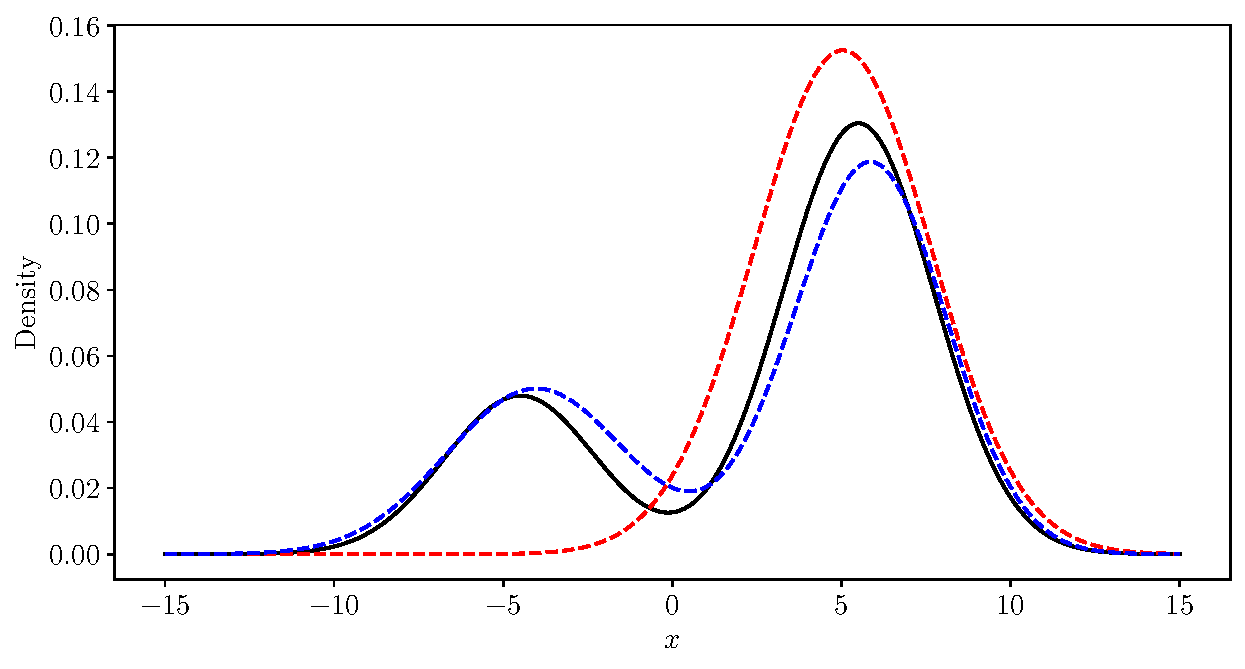
\includegraphics[width=\textwidth]{chp05_gmm/figures/bene_final_gmm}
	\caption{The mixture model algorithm implemented on Ben\^e's SDE \cref{eqn:bene_sde} with fixed initial condition \(x_0 = 0.5\) and over the time interval \((0,5)\).
		The probability density function of the true solution is shown in solid black and the corresponding linearisation solution in dashed red.
		The Gaussian mixture model density is overlaid in blue.
		A single split into three canonical sigma points (using \cref{eqn:uhlman_sigma} occurs at \(t = 0.8\)).}
	\label{fig:bene_gmm}
\end{figure}

As a simple example, we apply the algorithm to Ben\^e's SDE \cref{eqn:bene_sde}, subject again to the initial condition \(x_0 = 1/2\) and considered at the final time of \(t = 5\).
Recall from \cref{eqn:bene_sde_pdf} and \Cref{fig:bene_gauss} that the true solution has a bimodal density, which the Gaussian distribution resulting from a single linearisation is unable to capture.
We implement the Gaussian mixture model with a single split, manually chosen to be at time \(t = 0.8\), with the resulting mixture density shown in \Cref{fig:bene_gmm}.
The algorithm is initialised with \(x^{(1)} = 1/2\), \(\Sigma^{(1)} = 0\) and \(w^{(1)}\).
After propagating the initial condition by solving \cref{eqn:gauss_de} to the splitting time \(t = 0.8\), we use the canonical sigma points (\cref{eqn:uhlman_sigma}) to replace the Gaussian density with three points \(x^{(1)}, x^{(2)}, x^{(3)}\), preserving the mean and covariance.
We then propagate these three points forward separately, in that for each one we take the deterministic trajectory \(F_{0.8}^{5}\!\left(x^{(i)}\right)\) and compute the solution to the SDE \cref{eqn:bene_sde} linearised about this trajectory.
The result are three Gaussian distributions at \(t = 5\), which we then combine into a equally weighted sum to produce a Gaussian mixture model approximating the SDE solution.
In \Cref{fig:bene_gmm}, we compare the probability density function of the resulting Gaussian mixture model to the true solution density and the Gaussian approximation from a single linearisation.
Importantly, the mixture model density clearly includes two modes that resemble those of the true solution, which is an important feature of the solution that was not captured by the single linearisation.
Further configuration of the algorithm may result in a better fit; this was a simple and contrived example implemented to demonstrate the \emph{potential} of the mixture model algorithm in overcoming limitations of a single Gaussian approximation.
Computing the mixture model only required the propagation of 6 values---the three means and covariance values---by solving the pair \cref{eqn:gauss_de} of differential equations three times.
We are able to capture the bimodality, an important feature of the solution, with only a small number of calculations.
This would be particularly advantageous in a situation where the true solution is not analytically available (as in a majority of practical scenarios) and we would have to otherwise rely on bulk simulation to observe these features.

We can take this example further to attain a better fit, by adjusting the way in which the first Gaussian component is split.

% \td{Splitting}
% Similar algorithms combining linearisations and mixture models have been proposed, such as that by \citet{DeMarsEtAl_2013_EntropyBasedApproachUncertainty} for propagating an initial uncertainty through a non-linear model, which we compare to.
% However, such algorithms have seen little use in practice, particularly in the oceanography and climate modelling circles.
% In the following chapter (\Cref{ch:appls}), we will demonstrate the mixture model algorithm on examples from these domains.\lb{careful with this paragraph}

\section{The splitting criterion}\label{sec:gmm_split_disc}
In the implementation of our algorithm on Ben\^e's SDE, we manually chose a single split time.
However, in general the algorithm requires a choice of criterion for when to split a Gaussian component, for which there are several choices.
A given Gaussian component should be split when the linearised SDE is no longer a reasonable approximation for the original SDE about the deterministic trajectory corresponding to the component.
This requires an ongoing evaluation of the error in using the approximation.
Some possibilities include:
\begin{itemize}
	\item Alongside the propagation of the mixture model, one can also compute a small number of stochastic samples that solve the original SDE \cref{eqn:sde_y_gmm}.
	      These stochastic samples can be compared to the ongoing Gaussian evolutions, for instance using a probabilistic distance measure.
	      However, this would increase the computational load of the algorithm and may require many samples to accurately quantify departures from Gaussianity.
	      The Gaussian mixture model does provides an analytic probability density function that can lend itself to further inference, as opposed to solely stochastic samples that require an additional step to compute a density function.
	      There may be a trade-off between the number of samples and the desired computationally efficiency.

	\item A diagnostic based purely on the deterministic model will be computationally efficient, not requiring any stochastic simulation.
	      Stochastic sensitivity (introduced by \citet{Balasuriya_2020_StochasticSensitivityComputable} and extended in \Cref{sec:theory_s2}) is a scalar value that is computed directly from the covariance matrix of the Gaussian approximation, and quantifies the magnitude and direction of maximum uncertainty.
	      In highly nonlinear systems, stochastic sensitivity may provide a measure for evaluating non-Gaussianity.
	      This can be computed from each Gaussian component with minimal additional computational cost, by simply taking the operator norm of the component covariance matrix.
	      However, in regions of linearity and non-multiplicative noise, the solution to the SDE can be Gaussian, but stochastic sensitivity, being the magnitude of the noise, can increase.
	      A large value of stochastic sensitivity need to imply non-Gaussianity in these cases.


	\item \citet{DeMarsEtAl_2013_EntropyBasedApproachUncertainty} propose an algorithm for propagating an initial uncertainty through a nonlinear time-varying mapping, by using a Gaussian mixture model and a similar splitting algorithm.
	      The principle is similar to ours; the uncertainty is propagated forward using a linearisation of the model until this is no longer a reasonable approximation.
	      A split occurs when nonlinearity in the mapping, which would result in non-Gaussianity, is detected via an entropy-based measure.
	      This measure uses the sigma point method to evaluate the mapping of a covariance matrix, which is compared to the ongoing propagation of a Gaussian component.
	      The sigma point method provides an \emph{exact} computation for the covariance matrix of a deterministic nonlinear transformation of a random variable, provided that the transformation can be evaluated exactly.
	      In our case however, there is ongoing uncertainty from the multiplicative noise and the SDE cannot be solved exactly, so we cannot evaluate the mapping required for the sigma point method.
	      Nonetheless, this previous work may suggest a direction for further tuning the implementation of our method, including the selection of points when splitting a component.

\end{itemize}
We leave further development of this step of the algorithm for future work.




% \section{Error remains bounded}
% \note{THE PROBLEM: the mixture model at time \(t\) must be constructed from linearised SDEs all with the SAME Wiener process W_t. But then these solutions cannot possibly be independent. So the logic breaks down there.}
% \td{Check the following - important that all the linearisations used the same Wiener process. Why did I initially think this was wrong??}
% Our main result of \Cref{ch:linear_theory}, \Cref{thm:main}, establishes that the strong error in approximating the solution to a small-noise nonlinear stochastic differential equation with a linearisation is bounded by a scaling of the initial and ongoing uncertainty scales.
% In this section, we show that this result implies that if we propagate the components of a Gaussian mixture model with linearisations about the component means, as our mixture model algorithm employs, the error remains bounded in a similar fashion.

% Recall the results of \Cref{sec:theory_gauss}, the SDE linearisation theory in the special case of a Gaussian initial condition.
% Suppose that \cref{eqn:sde_no_eps} is subject to a Gaussian initial condition \(x \isGauss{\mu_0, \delta^2\Sigma_0}\), where \(\mu_0 \in \R^n\) and \(\Sigma_0 \in \R^{n\times n}\) are fixed and \(\delta > 0\) is a scaling parameter.
% We can linearise \cref{eqn:sde_no_eps} about the deterministic trajectory \(F_t^0\!\left(\mu_0\right)\) originating from the mean \(\mu_0\), as
% \begin{equation}
% 	\dif l_t\!\left(\mu_0, \delta^2\Sigma_0\right) = \begin{multlined}[t]
% 		\left[F_0^t\!\left(\mu_0\right) + \nabla u\!\left(F_0^t\!\left(\mu_0\right), t\right)\left(l_t\!\left(\mu_0, \delta^2 \Sigma_0\right) - F_0^t\!\left(\mu_0\right)\right)\right]\dif t \\
% 		+ \epsilon\sigma\!\left(F_0^t\!\left(\mu_0\right), t\right)\dif W_t, \quad l\!\left(\mu_0, \delta^2\Sigma_0\right) = x.
% 	\end{multlined}
% 	\label{eqn:scaled_sde_linear}
% \end{equation}
% We have temporarily adopted the notation \(l_t\!\left(\mu_0, \delta^2\Sigma_0\right)\) to indicate the dependence of the linearised solution on the initial mean and covariance matrix.
% The solution to \cref{eqn:scaled_sde_linear} at time \(t\) follows a Gaussian distribution with computable mean and covariance, specifically
% \[
% 	l_t\!\left(\mu, \delta^2\Sigma_0\right) \isGauss{F_0^t\!\left(\mu_0\right), \, \delta^2 \nabla F_0^t\!\left(\mu_0\right) \Sigma_0 \left[\nabla F_0^t\!\left(\mu_0\right)\right]^{\T} + \epsilon^2\Sigma_0^t\!\left(\mu_0\right)},
% \]
% where
% \[
% 	\Sigma_0^t\!\left(\mu_0\right) = \nabla F_0^t\!\left(\mu_0\right)\int_0^t{\left[\nabla F_0^\tau\!\left(\mu_0\right)\right]^{-1} \sigma\!\left(F_0^\tau\!\left(\mu_0\right), \tau\right)\sigma\!\left(F_0^\tau\!\left(\mu_0\right), \tau\right)^{\T}\left[\nabla F_0^\tau\!\left(\mu_0\right)\right]^{^{-\intercal}}\dif\tau}\left[\nabla F_0^t\!\left(\mu_0\right)\right]^{\T}.
% \]
% \Cref{thm:main} establishes that for any \(t \in [0,T]\), there exists constants \(A_1(t), A_2(t), A_3(t) \geq 0\) independent of \(\mu_0\) such that
% \begin{equation}\label{eqn:linear_error_bound}
% 	\avg{\norm{y_t - l_t\!\left(\mu_0, \delta^2 \Sigma_0\right)}} \leq A_1(t)\epsilon^2 + A_2(t)\epsilon\delta + A_3(t)\delta^2.
% \end{equation}
% Note that we have dropped the notation indicating the dependence of the constants on the coefficient bounds for notational brevity.
% Suppose at a time \(s < t\), we have a mixture model with \(M\) Gaussian components
% \[
% 	p_0\!\left(z\right) = \sum_{i=1}^{M}{\omega_i\Gauss{z;\, \mu_0^{(i)}, \delta^2\Sigma_0^{(i)}}}
% \]
% where \(\omega_1,\dotsc, \omega_M \geq 1\) are weights satisfying \(\sum_{i=1}^M{\omega_i} = 1\), \(\mu_0^{(1)}, \dots \mu_0^{(M)}\) are the component means and \(\Sigma_0^{(1)}, \dotsc, \Sigma_0^{(M)}\) are the component covariance matrices.
% Via linearisation approximations of the form \cref{eqn:scaled_sde_linear}, we construct the mixture model at time \(t > s\)
% \[
% 	p_t\!\left(z\right) = \sum_{i=1}^{M}{\omega_i\Gauss{z; \, F_s^t\!\left(\mu_0^{(i)}\right), \Pi^{(i)}}},
% \]
% where
% \[
% 	\Pi^{(i)} = \delta^2 \nabla F_0^t\!\left(\mu_0\right) \Sigma_0^{(i)} \left[\nabla F_s^t\!\left(\mu_0\right)\right]^{\T} + \epsilon^2 \Sigma_s^t\!\left(\mu_0\right),
% \]
% is the propagated covariance matrix.
% Let \(\Xi_0\) be a random variable distribution distributed according to \(p_0\), which we can write as
% \[
% 	\Xi_0 = \sum_{i=1}^{M}{I_i \xi_0^{(i)}}
% \]
% where \(\xi_0^{(i)} \isGauss{\mu_0^{(i)}, \Sigma_0^{(i)}}\) independently for each \(i\), and \(\left(I_1, \dotsc, I_M\right)\) are a set of indicator variables with
% \[
% 	P\!\left(I_i = 1,\, I_j = 0 \text{ for all } j \neq i\right) = \omega_i,
% \]
% for each \(i = 1,\hdots,M\), and zero probability otherwise.
% Similarly, let \(\Xi_t\) be a random variable distributed according the mixture model \(p_t\), which we construct from solutions to linearised SDEs of the form \cref{eqn:scaled_sde_linear}, by writing
% \[
% 	\Xi_t = \sum_{i=1}^{M}{I_i l_t\!\left(\mu_0^{(i)}, \delta^2\Sigma_0^{(i)}\right)},
% \]
% where each solution to \cref{eqn:scaled_sde_linear} is independent of the others.
% Then, for any \(i\) we have the conditional distribution
% \[
% 	\left. \Xi_t \, | \, \set{I_i = 1, \, I_j = 0 \text{ for all } j \neq i} \right. = l_{t}\left(\mu_0^{(i)}, \delta^2 \Sigma_0^{(i)}\right).
% \]
% The random variable \(\Xi_t\) represents our approximation of the state at time \(t\), after a single step of the mixture model algorithm.
% Via the law of total expectation, the error in approximating \(y_t\) with \(\Xi_t\) is
% \begin{align*}
% 	\avg{\norm{y_t - \Xi_t}} & = \sum_{i=1}^{M}{\avg{\norm{y_t - \Xi_t}\,\middle|\, I_i = 1}}P\!\left(I_i = 1,\, I_j = 0 \text{ for all } j \neq i\right) \\
% 	                         & = \sum_{i=1}^{M}{\omega_i\avg{\norm{y_t - l_{t}\left(\mu_0^{(i)}, \delta^2 \Sigma_0^{(i)}\right)}}}                        \\
% 	                         & = \sum_{i=1}^{M}{\omega_i\left(A_1(t)\epsilon^2 + A_2(t) \epsilon \delta + A_3(t)\delta^2\right)}                          \\
% 	                         & = A_1(t) \epsilon^2 + A_2(t)\epsilon\delta + A_3(t)\delta^2.
% \end{align*}
% In the mixture model algorithm described, the initialising uncertainty (being a component of the mixture model) at each step scales with \(\epsilon\), specifically \(\delta = \epsilon\).
% Thus, the error in the algorithm remains bounded with order \(\epsilon^2\).
% Note that each linearised SDE of the form \cref{eqn:scaled_sde_linear} is driven by the same Wiener process \(W_t\) as the original nonlinear SDE \cref{eqn:sde_y_gmm}.


% \td{Explain that further theory is needed}
